\begin{figure*}
	\centering
	\begin{subfigure}[t]{0.5\textwidth}
		\centering
		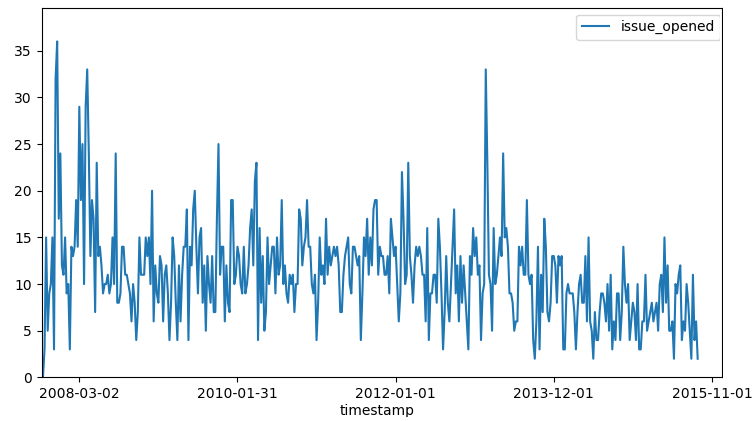
\includegraphics[width=\linewidth]{images/sample/sample_raw.png}
		\caption{Number of issues raised on a weekly basis from 2008 to 2014.}
		\label{fig:sample_raw}
	\end{subfigure}%
	~
	\begin{subfigure}[t]{0.415\textwidth}
		\centering
		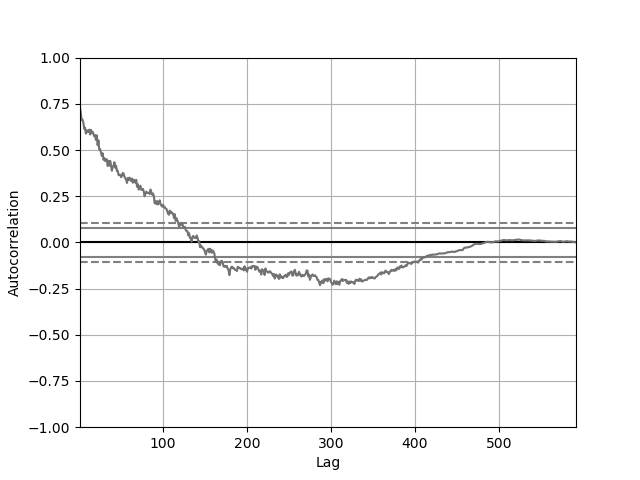
\includegraphics[width=\linewidth]{images/sample/sample_autocorr.png}
		\caption{Autocorrelation plot of issue reports. The ``lag'' parameter indicates the number of weeks over which the autocorrelation was computed. Note that autocorrelation is significantly large for lag$\geq$20 weeks.}
		\label{fig:sample_autocorr}	
	\end{subfigure}%
	\\
	\begin{subfigure}[t]{0.57\textwidth}
		\centering
		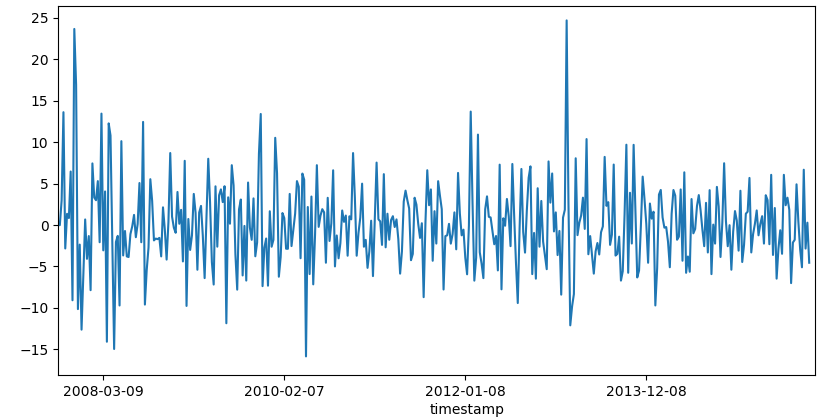
\includegraphics[width=\linewidth]{images/sample/sample_mre.png}
		\caption{Residual error of ARIMA estimate measured as $E=Y-\hat{Y}$. Note that the largest residual error is less that 25. This indicates a relatively accurate model.}
		\label{fig:sample_resid}	
	\end{subfigure}%
	~
	\begin{subfigure}[t]{0.4\textwidth}
		\centering
		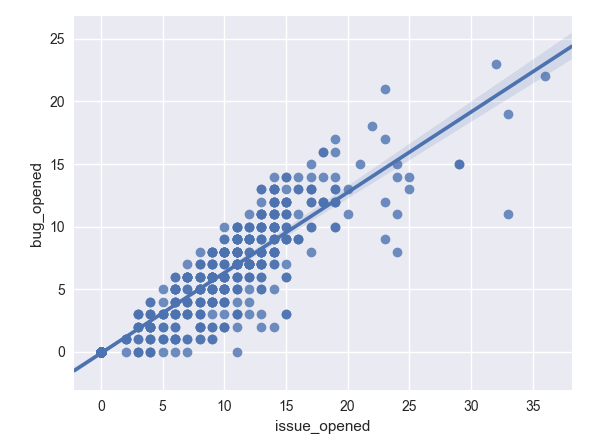
\includegraphics[width=\linewidth]{images/sample/sample_corr.png}
		\caption{Correlation between issues raised and bugs reported. Note the existence of a strong correlation between \#issues and \#bugs.}
		\label{fig:sample_corr}	
	\end{subfigure}%
	\caption{Motivating example: Time Series Analysis of issue reports for ArangoDB from 2008 to 2014.}
	\label{fig:ArangoDB}
\end{figure*}
